\section{Results} \label{sec:results}
Here the results will be presented. We start taking a look at how good our linear regression is, by fitting a polynomial to points drawn from a known PDF. Thereafter we will see how good the regression is when using real terrain data. To give a intuition on how good the fit is, we will in both cases how 3D plots of the graphs using various methods, and then present the error analysis. 

\subsection{Franke function}
Below one can find the results of the regression on Franke function

\subsubsection{Visualization of graphes}
In figure \eqref{fig:franke} one can find a 3D visualization of the Franke function, for easier comparison with the fitted graphs presented in figure \eqref{fig:franke_plots}. The data sets were composed drawing random $x$'s and $y$'s in the interval $x,y\in[0,1]$ from a uniform distribution, and the corresponding $z$-values where obtained from the Franke function. Further, we added noise produced by $\mathcal{N}(0, \sigma^2=0.1)$ and compared with the undisturbed data set. For Lasso and Ridge, we used a penalty $\lambda=1e-15$, and for Lasso we also used gradient descent for minimization. On that occasion, the learning rate was set to $\eta=0.001$ with niter$=1000000$ as the number of iterations. 
 \begin{figure} [h]
 	\centering
 	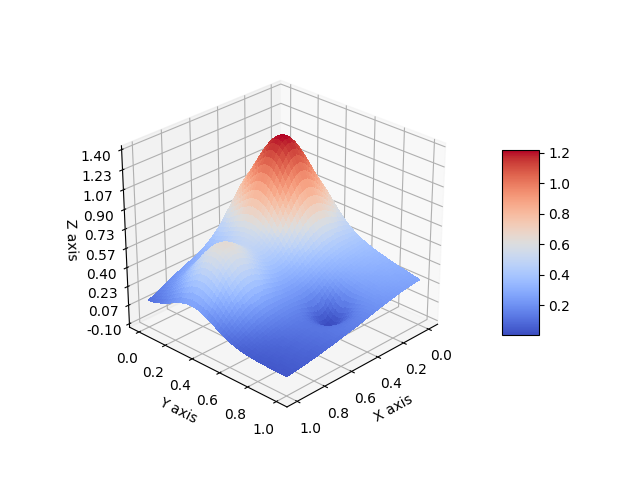
\includegraphics[scale=0.8]{../plots/franke.png}
 	\caption{The Franke function in the interval $x\in[0,1]$, $y\in[0,1]$, $z\in[0, 1.2]$.}
 	\label{fig:franke}
 \end{figure}

 
\newgeometry{left=2cm,right=2cm,top=1cm}
\begin{figure} [H]%
    \centering
    \subfloat[OLS without noise]{{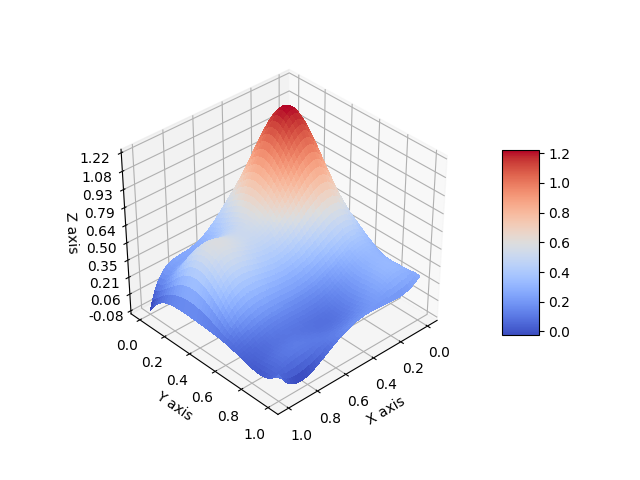
\includegraphics[width=9cm]{../plots/OLS.png} }}%
    \subfloat[OLS with noise]{{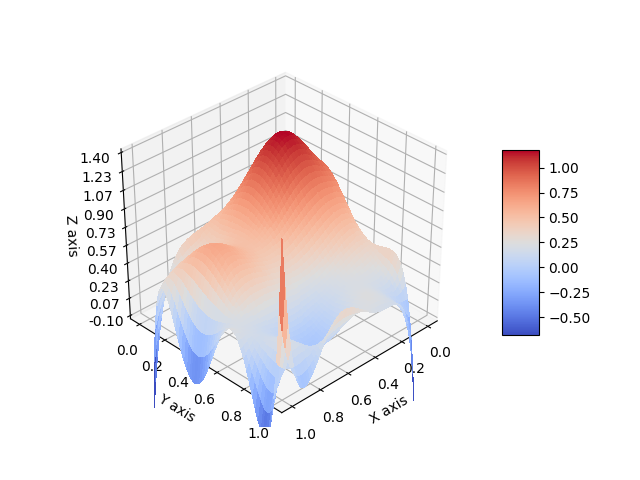
\includegraphics[width=9cm]{../plots/OLS_noise.png} }}\\

    \subfloat[Ridge without noise]{{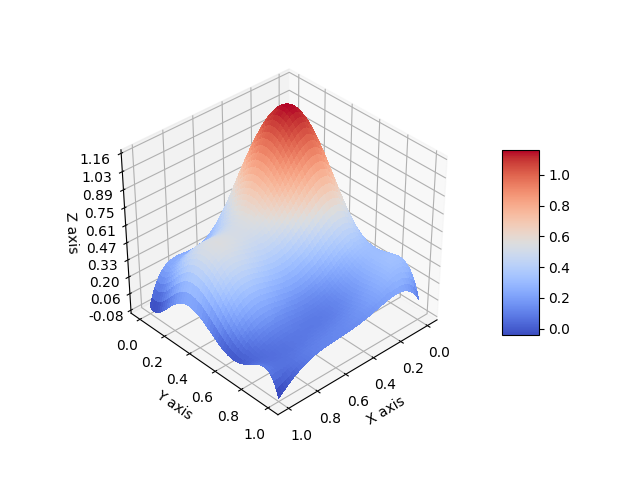
\includegraphics[width=9cm]{../plots/Ridge.png} }}%
    \subfloat[Ridge with noise]{{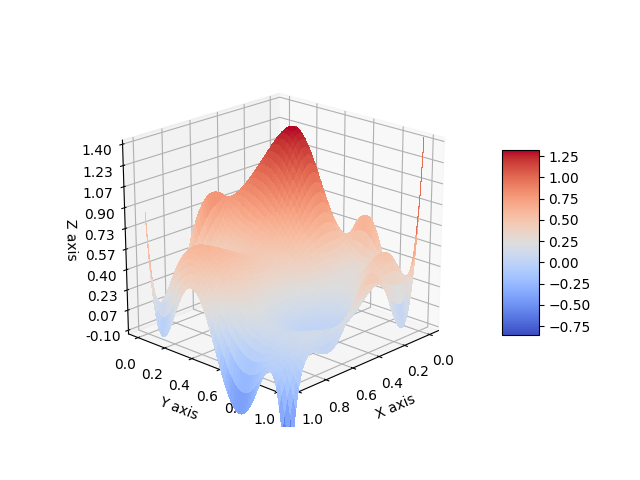
\includegraphics[width=9cm]{../plots/Ridge_noise.png} }}\\
    
    \subfloat[Lasso without noise]{{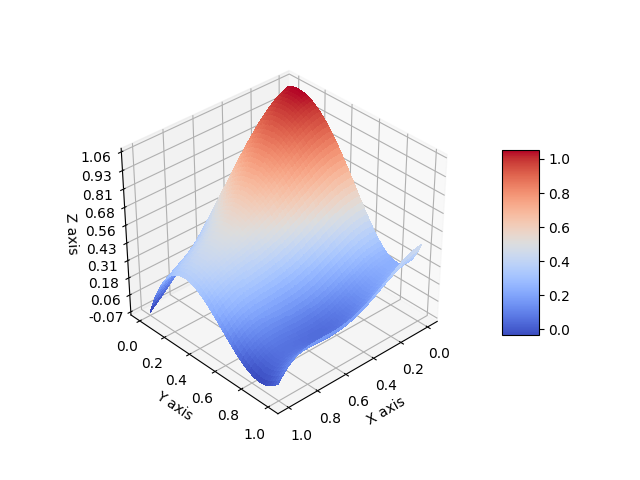
\includegraphics[width=9cm]{../plots/Lasso.png} }}%
    \subfloat[Lasso with noise]{{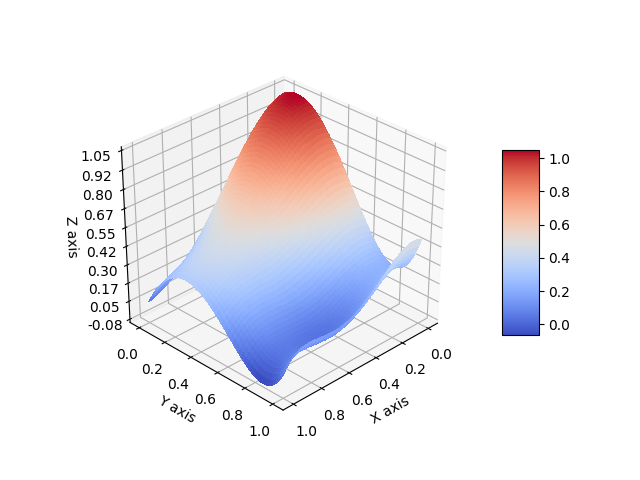
\includegraphics[width=9cm]{../plots/Lasso_noise.png} }}
    \caption{Fitted polynomial by OLS, Ridge and Lasso with and without noise. For Ridge and Lasso, we used a low penalty of $\lambda=1e-15$. Lasso was performed with $\eta=1e-3$ and 1e6 iterations. The noise was sampled from a normal distribution with $\sigma=0.1$.}%
    \label{fig:franke_plots}%
\end{figure}

\restoregeometry

\begin{figure} [H]%
	\centering
	\subfloat[OLS self]{{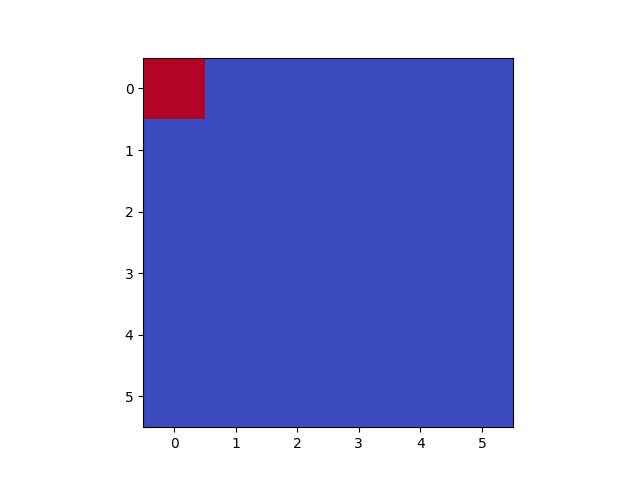
\includegraphics[width=3cm]{../plots/beta_ols_visualize.png} }}%
	\subfloat[Ridge self]{{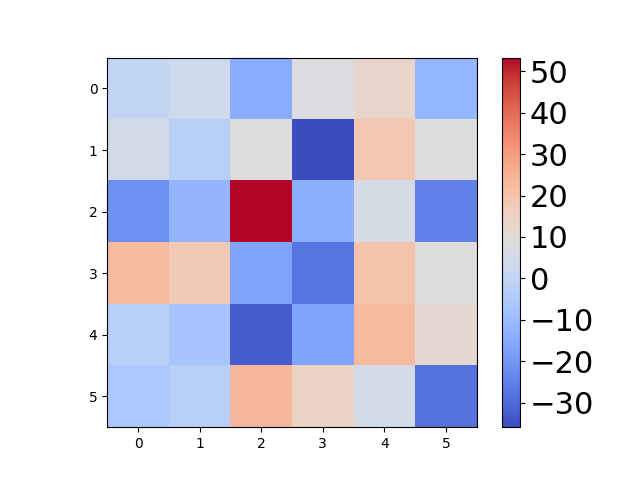
\includegraphics[width=3cm]{../plots/beta_ridge_visualize.png} }}%
	\subfloat[Lasso self]{{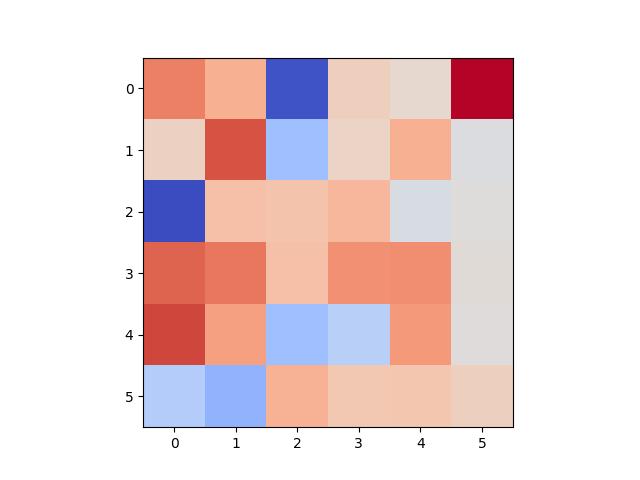
\includegraphics[width=3cm]{../plots/beta_lasso_visualize.png} }}%
	\subfloat[Ridge2 self]{{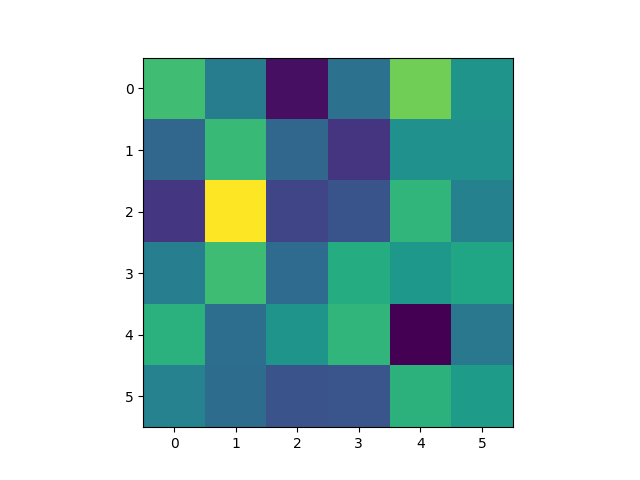
\includegraphics[width=3cm]{../plots/beta_ridge2_visualize.png} }}\\
	
	\subfloat[OLS scikit]{{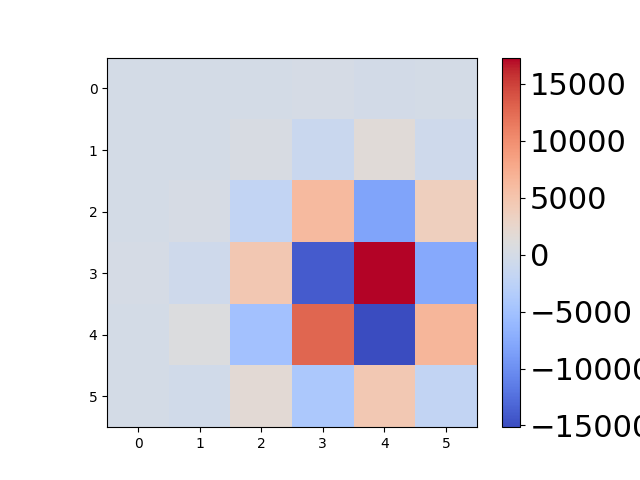
\includegraphics[width=3cm]{../plots/beta_ols_test_visualize.png} }}%
	\subfloat[Ridge scikit]{{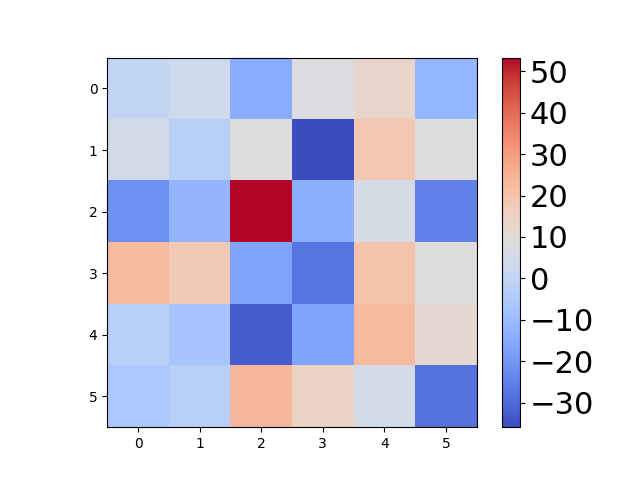
\includegraphics[width=3cm]{../plots/beta_ridge_test_visualize.png} }}%
	\subfloat[Lasso scikit]{{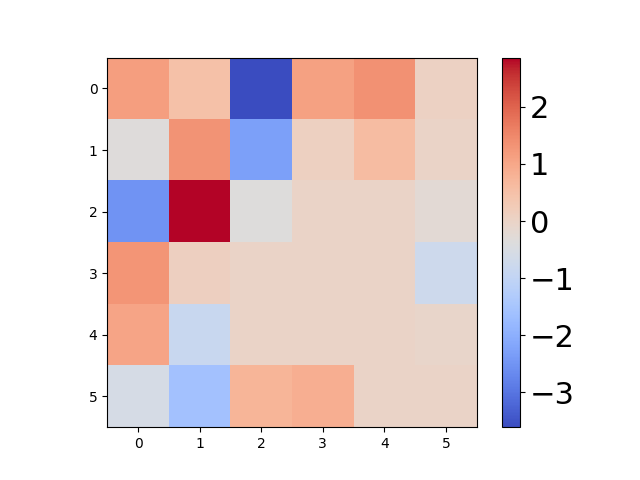
\includegraphics[width=3cm]{../plots/beta_lasso_test_visualize.png} }}%
	\subfloat[Ridge scikit]{{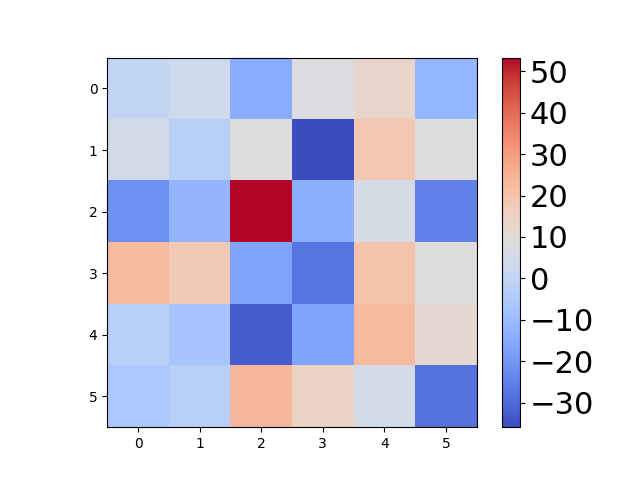
\includegraphics[width=3cm]{../plots/beta_ridge_test_visualize.png} }}
	
	\caption{}%
	\label{fig:beta_plots}%
\end{figure}

\begin{figure} [H]%
	\centering
	\subfloat[OLS without noise]{{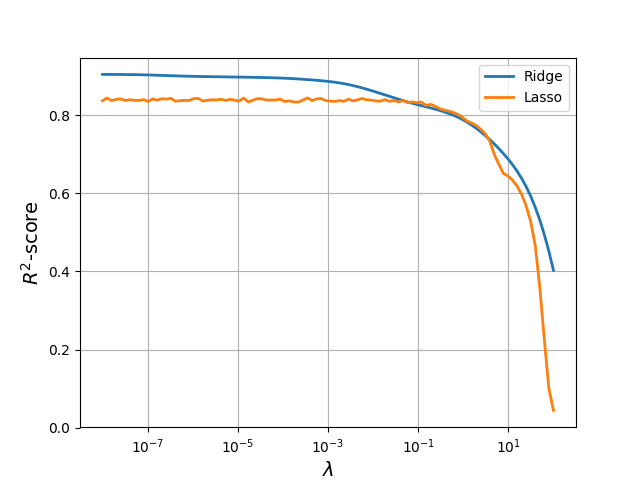
\includegraphics[width=8cm]{../plots/lambda_R2score.png} }}%
	\subfloat[OLS with noise]{{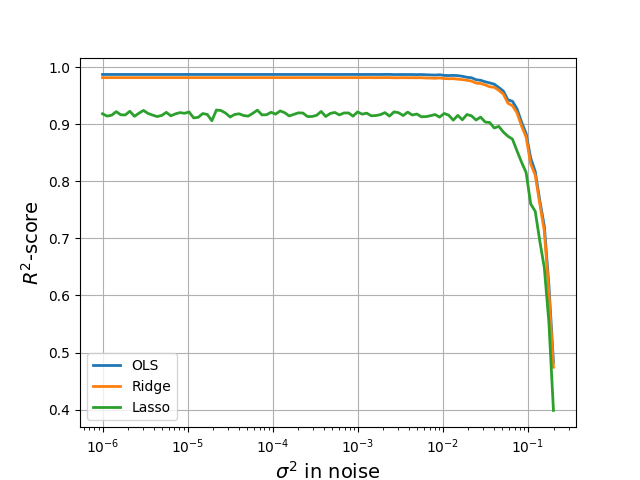
\includegraphics[width=8cm]{../plots/var_R2score.png} }}
	\caption{}%
	\label{fig:R2_scores}
\end{figure}

\subsubsection{Error}

\begin{table} [H]
	\caption{Write table text here.  \vspace{2mm}}
	\begin{tabularx}{\textwidth}{l|XX|XX} \hline\hline
		\label{tab:franke_error}
		& \multicolumn{2}{c}{\textbf{MSE}}&\multicolumn{2}{c}{\textbf{R2}}\\ \hline
		&self&scikit&self&scikit\\ \hline \\
		OLS & 0.07853 & 0.86104 & 0.05386 & 1.7483\\
		Ridge & 0.07852 & 0.86410 & 0.05406 & 1.6904 \\
		Lasso & 0.07704 & 0.86231 & 0.07187 & 1.6492 \\
		RidgeGD & 0.07523 & 0.91850 & 0.09362 & 1.3217 \\ \hline
	\end{tabularx}
\end{table}


-Vary $\lambda$ and the noise\\
-MSE and R2\\
-Resampling



\subsection{Real data}
First we will take a look at how good our linear regression is...
\subsubsection{Visualization of graphes}

 \begin{figure} [H]
 	\centering
 	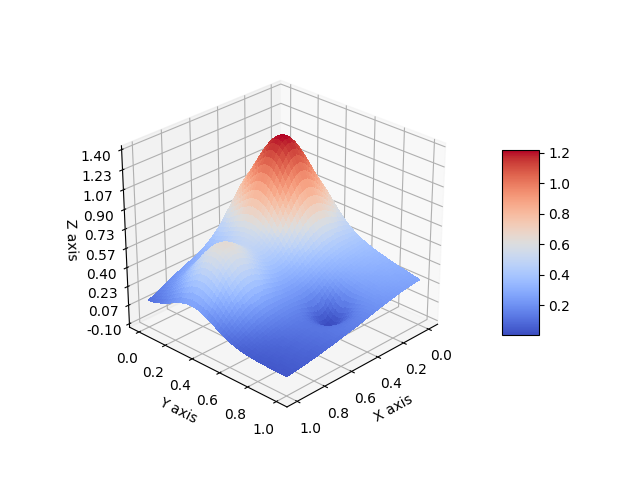
\includegraphics[scale=0.8]{../plots/franke.png}
 	\caption{The Franke function in the interval $x\in[0,1]$, $y\in[0,1]$, $z\in[0, 1.2]$.}
 	\label{fig:franke2}
 \end{figure}

 
\newgeometry{left=2cm,right=2cm,top=1cm}
\begin{figure} [H]%
    \centering
    \subfloat[OLS without noise]{{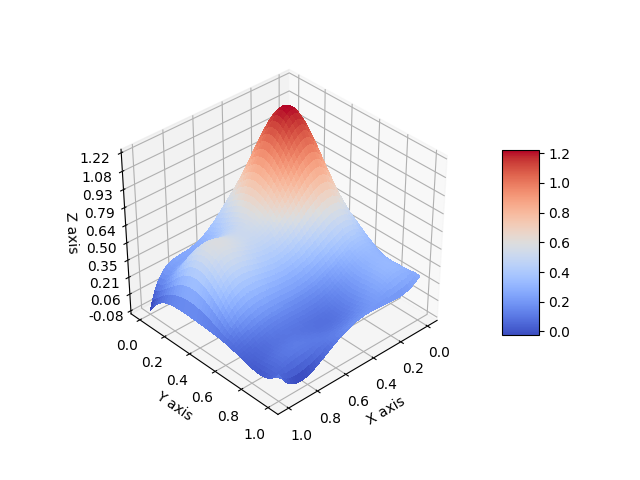
\includegraphics[width=9cm]{../plots/OLS.png} }}%
    \subfloat[OLS with noise]{{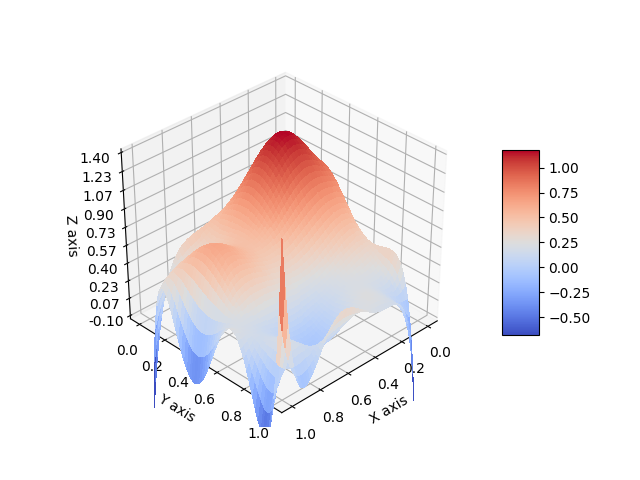
\includegraphics[width=9cm]{../plots/OLS_noise.png} }}\\

    \subfloat[Ridge without noise]{{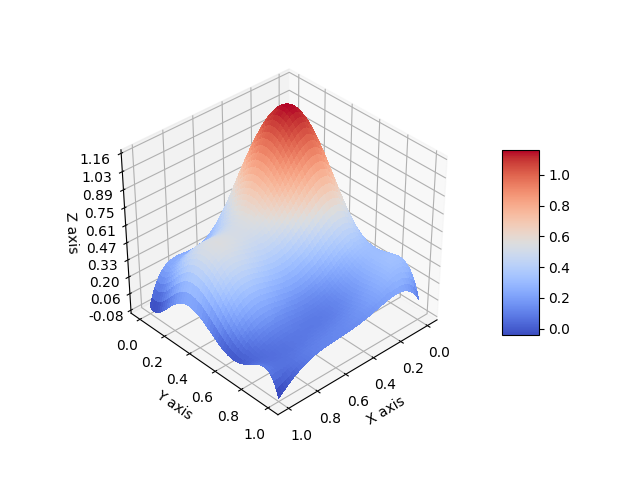
\includegraphics[width=9cm]{../plots/Ridge.png} }}%
    \subfloat[Ridge with noise]{{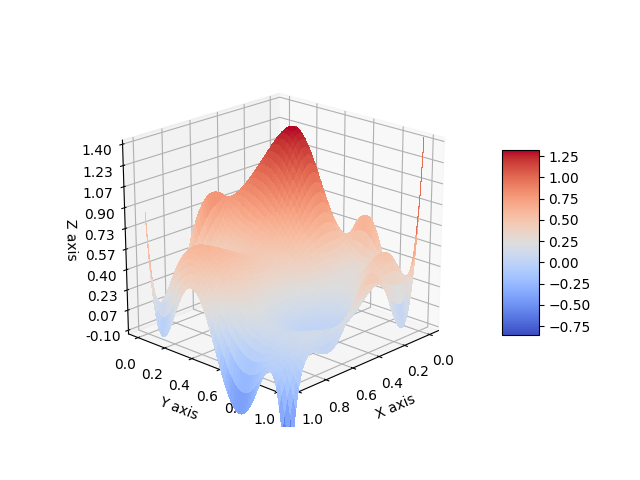
\includegraphics[width=9cm]{../plots/Ridge_noise.png} }}\\
    
    \subfloat[Lasso without noise]{{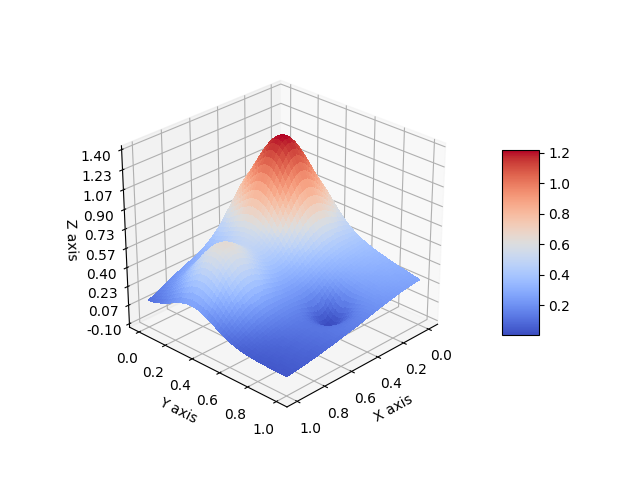
\includegraphics[width=9cm]{../plots/franke.png} }}%
    \subfloat[Lasso with noise]{{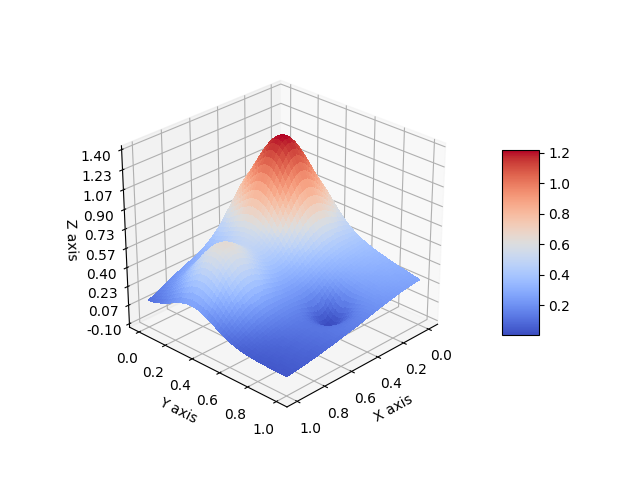
\includegraphics[width=9cm]{../plots/franke.png} }}
    \caption{Fitted polynomial by OLS, Ridge and Lasso with and without noise. For these plots, we used a low penalty of $\lambda=1e-15$.}%
    \label{fig:example}%
\end{figure}

\subsubsection{Error}

